\documentclass[conference]{IEEEtran}
\usepackage{amsmath, amssymb, amsfonts}
\usepackage{algorithmic}
\usepackage{graphicx}
\usepackage{tabularx}
\usepackage{booktabs}
\usepackage{multirow}
\usepackage[table]{xcolor}
\usepackage{hyperref}
\usepackage{listings}
\usepackage{xcolor}
\usepackage{url}
\usepackage{cite}
\lstset{
    basicstyle=\footnotesize\ttfamily,
    breaklines=true,
    frame=single,
    language=Python
}

\title{Athlyze – An Agentic RAG Approach for Personalized Fitness and Nutrition}
\author{
    \IEEEauthorblockN{Nishchay Patel}
    \IEEEauthorblockA{
        Department of Computer Science, \\ 
        Georgia State University,\\
        Atlanta, GA, USA\\
        \href{mailto:npatel237@student.gsu.edu}{npatel237@student.gsu.edu}
    }
}

\begin{document}

\maketitle

\begin{abstract}
Current fitness and nutrition applications often rely on rigid algorithms and static models, limiting their ability to provide personalized and data-driven recommendations. This paper introduces Athlyze, a novel system that leverages Agentic Retrieval-Augmented Generation (RAG) to enhance fitness and nutrition guidance through dynamic, research-backed insights. Unlike conventional applications, which provide generic advice based on predefined models, Athlyze integrates a vector database populated with embeddings from scientific literature on muscle development and nutrition. By employing clustering algorithms and adaptive recommendation models, Athlyze tailors its guidance to individual user profiles, optimizing dietary and fitness plans based on evolving data. Implemented using GCP tools, GEMINI, LangFlow, and AstraDB, the system refines retrieval processes and improves recommendation accuracy over time. Our findings demonstrate that an agentic RAG-based approach not only enhances personalization but also establishes a scalable and intelligent framework for data-driven health optimization. Future work will focus on refining retrieval techniques, optimizing model performance, and expanding the research database, with iterative user testing guiding development.\\
\end{abstract}

\renewcommand\IEEEkeywordsname{Keywords}
\begin{IEEEkeywords}
RAG, Agentic RAG, Semantic Chunking, Fitness Applications, Vector Databases, Context Preservation, Prompt Engineering, Langflow, Personalized Nutrition
\end{IEEEkeywords}

\section{introduction}
The increasing demand for personalized fitness and nutrition solutions has exposed the limitations of traditional applications, which rely on static algorithms and predefined templates. These conventional systems fail to consider the complexities of individual physiology, dietary needs, and training goals, often leading to generic recommendations that lack scientific rigor\cite{9}. Research highlights that customized fitness and nutrition plans significantly improve adherence and outcomes, yet most existing applications, such as MyFitnessPal and Fitbit, depend on rule-based methodologies that overlook dynamic, research-backed insights.

Athlyze presents an Agentic Retrieval-Augmented Generation (RAG) solution that bridges this gap by integrating scientific literature and machine learning-driven personalization into a cohesive system. Unlike conventional fitness applications, Athlyze utilizes a vector database embedded with research papers on muscle development, nutrition, and physical training principles, allowing users to receive tailored, evidence-based recommendations \cite{5}. By incorporating clustering algorithms, regression models, and adaptive recommendation systems, Athlyze dynamically adjusts fitness and dietary plans to align with user profiles, optimizing outcomes based on scientific data and real-time feedback.

Preliminary studies suggest that AI-driven recommendation systems enhance engagement and adherence rates by over 30\%, demonstrating the value of machine learning and NLP in health optimization \cite{10}. Athlyze builds on this by employing Google Cloud Platform (GCP), GEMINI, LangFlow, and AstraDB, ensuring a scalable and efficient implementation for retrieval-augmented recommendations. By combining semantic search with ML-driven user segmentation, Athlyze refines its guidance over time, making it a comprehensive, research-backed approach to fitness and nutrition planning.

Beyond personalization, Athlyze advances the intersection of AI, fitness, and nutritional science, providing users with real-time, research-driven insights into training methodologies and dietary principles. This study explores the scalability and effectiveness of an Agentic RAG-based system in transforming physical training and nutrition planning, paving the way for a data-driven, adaptive approach to muscle-building and health optimization.

Athlyze resolves this through a neurosymbolic architecture combining:

\begin{itemize}
    \item Agentic chunking with dynamic sentence handling
    \item Research backed guidelines
    \item Real-time adaptation using Google language models
    \item Reasoning the response for the user against the research database
\end{itemize}

The rising demand for personalized health solutions has exposed the limitations of conventional fitness applications, which rely on predefined templates and generic algorithms. Such systems typically fail to account for individual differences in demographics, goals, and constraints. Recent advances in machine learning (ML) and natural language processing (NLP), particularly in Retrieval-Augmented Generation (RAG), offer immense potential to bridge this gap.

\section{limitations of existing methods}\

Current fitness and nutrition applications rely on predefined algorithms and static models, limiting their ability to deliver personalized, data-driven insights. These traditional approaches struggle to adapt to individual user needs, often resulting in generic recommendations that fail to account for variations in physiology, diet, and fitness goals.

\subsection{limitations of conventional fitness applications}

Users relying on existing fitness applications encounter several inefficiencies that hinder effectiveness and validation:\\

\begin{itemize}
	\item Rigid Algorithmic Models: Most fitness platforms use rule-based heuristics that fail to dynamically adapt to evolving user progress, dietary habits, or exercise performance. This results in stagnant recommendations that do not reflect real-time needs.
	\item Lack of Scientific Integration: Existing applications seldom incorporate peer-reviewed research on nutrition, muscle development, and exercise physiology, leading to recommendations that may not align with scientific best practices. \cite{7}
	\item One-Size-Fits-All Approach: Most fitness apps segment users into broad categories rather than leveraging granular, personalized insights. This lack of adaptive learning results in suboptimal fitness plans and nutritional guidance.
	\item User Drop-off Due to Frustration: Inaccurate or overly generalized recommendations often cause users to disengage, leading to low retention rates and decreased motivation. \cite{8}
        \item This limitation can be represented mathematically as:
            \begin{equation}
            \text{Error Rate} \propto \frac{\text{Static Templates}}{\text{Research Integration}} \times \text{User Complexity}
\end{equation}
\end{itemize}

\subsection{inadequate data extraction and cleaning}  
Initial attempts with conventional tools revealed critical flaws:  

\begin{table}[h]  
\caption{Text Extraction Performance Comparison}  
\begin{tabularx}{\linewidth}{lcc}  
\toprule  
\textbf{Metric} & \textbf{PyPDF2} & \textbf{Google Document AI} \\  
\midrule  
Structural Preservation & 43\% & 78\% \\  
Table Recognition & 12\% & 67\% \\  
Error Rate & 18\% & 9\% \\  
Processing Time (Large Docs) & Fast & Slow \\  
\bottomrule  
\end{tabularx}  
\end{table}  

Traditional tools, such as PyPDF2 and Google Document AI, struggle with extracting structured data from complex academic documents. These limitations include:  

\begin{itemize}  
    \item Loss of Document Structure: Section headers, figures, equations, and footnotes are often not preserved, leading to disorganized outputs.  
    \item Formatting Issues: Extracted text frequently contains irregular line breaks, spacing errors, and misplaced elements.  
    \item Incomplete Extraction: Tables and graphical content are often ignored or extracted incorrectly, reducing data reliability.  
    \item Google Document AI Limitations: While more advanced, it has restrictions on document size and takes significantly longer to process large academic papers.  
\end{itemize}  

These challenges highlight the need for a more efficient and structurally aware data extraction approach.  

\subsection{static chunking failures}  
Fixed-size chunking methods in conventional data processing cause significant semantic fragmentation:  

\begin{equation}  
\text{Fragmentation Score} = \frac{\text{Disconnected Concepts}}{\text{Total Chunks}} \times 100  
\end{equation}  

Traditional approaches often segment text arbitrarily, leading to:  

\begin{itemize}  
    \item Loss of Crucial Context: Key concepts are split across chunks, reducing comprehension and context retention (context preservation only 52\%).  
    \item Inability to Adapt to Query Variability: Fixed chunking does not account for dynamically changing user inputs or research content, leading to disjointed retrieval results.  
\end{itemize}  

These limitations hinder effective information extraction and retrieval, making conventional methods unsuitable for complex, research-driven applications.  

\subsection{scientific disconnect}
Existing systems demonstrate poor or no integration with scientific literature, significantly limiting evidence-based decision-making and suggestions for the user.\\

These challenges highlight the need for adaptive chunking and scientifically grounded retrieval mechanisms to improve information relevance and accuracy.  

\section{retrieval-augmented generation (rag)}

Retrieval-Augmented Generation (RAG) is a versatile framework in natural language processing (NLP) that combines the capabilities of information retrieval systems with generative models to enhance the quality and relevance of generated text. Unlike traditional approaches that rely solely on generative models or retrieval systems, RAG integrates both methods to create responses grounded in external knowledge while maintaining the flexibility of language generation. \cite{1} \cite{2}

\subsection{key components of rag}

\begin{itemize}
\item \textbf{Information Retrieval:} Extracts relevant data or text from external knowledge sources, ensuring responses are contextually informed.
\item \textbf{Representation of Knowledge:} Converts retrieved information into representations that can be effectively utilized during the generation process.
\item \textbf{Integration with Language Generation:} Seamlessly incorporates retrieved knowledge into the generative pipeline to produce coherent and meaningful outputs.\\
\end{itemize}

\begin{figure}[h!]
    \centering
    \includegraphics[width=0.95\linewidth]{RAG.png}
    \caption{Naive RAG (adapted from \cite{12}).}
    \label{fig:RAG}
\end{figure}


\begin{itemize}
\item \textbf{Irrelevant Retrieval:} RAG systems often struggle to filter out irrelevant or tangential data retrieved from external sources. This can lead to responses that, while coherent, fail to directly address user queries or provide actionable insights, which is critical for Athlyze's focus on precise academic or administrative inquiries.
\item \textbf{Lack of Iterative Reasoning:} Current RAG implementations lack robust iterative reasoning capabilities. This limitation can hinder the system's ability to handle complex, multi-step questions, which may be essential for Athlyze's domain-specific requirements.
\item \textbf{Ambiguity in Responses:} Responses generated by RAG can sometimes be vague or overly general, especially when the retrieved context is insufficiently integrated into the output. This can confuse users who need clear and detailed answers
\item \textbf{Hallucination:} Traditional RAG exhibited around 23\% hallucination rates.\\

\end{itemize}

\section{agentic retrieval-augmented generation}

Agentic Retrieval-Augmented Generation (RAG) represents a significant advancement in retrieval-based AI systems, integrating retrieval mechanisms with generative models to provide more contextually relevant and semantically accurate outputs. Unlike traditional RAG frameworks, which operate with static chunking and predefined retrieval structures, the agentic approach dynamically adapts to input variations, optimizing content retrieval and synthesis in real time.  

Building on IBM’s principles of agentic chunking, this approach ensures that information is structured in a way that enhances both retrieval precision and generative consistency. The key methodologies enabling this refinement include:

\begin{itemize}
    \item \textbf{Dynamic Proposition Handling:} Adjusts chunk boundaries in response to the evolving context, ensuring that retrieved segments maintain logical and semantic integrity. This adaptive mechanism enhances the system’s ability to generate coherent responses by preserving meaningful relationships between data points. \cite{12}
    \item \textbf{Metadata-Enriched Segmentation:} Incorporates structured metadata—such as content type, source credibility, temporal attributes, and hierarchical positioning—into chunked segments. This additional layer of information enhances retrieval efficiency by allowing models to weigh contextual importance during generation. \cite{4}
    \item \textbf{Recursive Merging:} Employs an iterative approach to combine semantically similar chunks, preventing fragmentation of related concepts. By utilizing an optimal similarity threshold ($\alpha=0.63$), RAG systems ensure that information is aggregated in a way that maintains coherence without diluting specificity. \cite{13}
\end{itemize}

These foundational techniques empower RAG systems to retrieve and generate responses that are more accurate, context-aware, and semantically aligned with user queries. Additionally, the integration of agentic chunking plays a critical role in refining data processing by:

\begin{itemize}
    \item \textbf{Optimized Chunking Strategy:} Unlike static chunking, agentic chunking dynamically determines optimal segment boundaries, ensuring that each text fragment is neither too granular nor excessively broad. This enhances both retrieval effectiveness and generative fluency. \cite{3}
    \item \textbf{Adaptive Context Management:} By continuously analyzing incoming queries and retrieved knowledge, the system dynamically refines retrieval strategies, prioritizing the most contextually relevant information while filtering out redundancies or unrelated content.
    \item \textbf{Efficient Knowledge Integration:} The structured combination of retrieved documents and user-specific queries results in a knowledge synthesis process that improves response consistency and factual accuracy.
\end{itemize}

Through these innovations, Agentic RAG enhances both the efficiency and accuracy of retrieval-augmented systems, making it particularly valuable for domains requiring complex knowledge synthesis, such as legal research, academic inquiry, and domain-specific AI assistants. By enabling more precise retrieval, structured knowledge representation, and adaptive generative capabilities, RAG systems powered by agentic principles push the boundaries of contextual AI applications.

\begin{figure}[h!]
    \centering
    \includegraphics[width=0.95\linewidth]{AgenticRAG.png}
    \caption{Agentic RAG (adapted from \cite{12}).}
    \label{fig:RAG}
\end{figure}


\section{proposed approach}
Athlyze integrates multiple modules into a cohesive and parallel pipeline designed to enhance fitness and nutrition recommendations. The system follows two parallel structured agentic AI workflow to ensure scientifically accurate fitness recommendations through controlled generative outputs with quicker throughput. The overall steps revolving around the entire application are:

\subsection{data and text preprocessing}
The data preprocessing pipeline is critical for ensuring the accuracy of the extracted information. The text is to be collected from around 10 research papers each in muscle and nutrition domain.

\begin{itemize}
    \item Initial attempts using traditional tools such as PyPDF2 and Google Document AI proved inadequate due to structural loss and formatting issues.
\end{itemize}

\textbf{Semantic Chunking:}
Traditional fixed-size chunking techniques were replaced by a more adaptive approach to preserve contextual meaning:
\begin{itemize}
    \item \textbf{Agentic Chunking with Gemini:} Dynamically adjusts chunk boundaries based on semantic relevance and user behavior, ensuring better content continuity.
\end{itemize}

\begin{lstlisting}[language=Python]
class AgenticChunker:
    def _find_relevant_chunk(self, proposition):
        prompt = ChatPromptTemplate.from_messages([
            ("system", "Determine statement relevance (yes/no):"),
            ("user", f"Existing: {existing_props}\New: {proposition}")
        ])
        return 'yes' in Gemini(prompt).content.lower()
\end{lstlisting}

\subsection{embedding generation and vector db integration}
The preprocessing stage leads into embedding generation, facilitating the creation of a robust and efficient search and retrieval system.

\textbf{Embedding Generation:}
\begin{itemize}
    \item Uses Google AI's `text-embedding-004` to convert text chunks into 768-dimensional vectors, which capture the semantic meaning of the text.
    \item Batch processing is optimized, with 50 chunks processed per API call, including error handling and exponential backoff strategies to ensure smooth operations.
\end{itemize}

\textbf{AstraDB Integration:}
The research repository is stored in AstraDB, embedding 1,703 rows of muscle training and 3,858 rows of nutrition research papers using Google's text-embedding-004 model. To optimize retrieval:
\begin{itemize}
    \item Each record contains the vector embedding, a unique ID, metadata, and text extracted from various research papers to support efficient retrieval.
\end{itemize}

\begin{table}[h]
    \caption{Representation of the Database}
    \centering
    \small % Use smaller font size instead of resizing
    \begin{tabular}{|c|c|p{2.4cm}|}
        \hline
        \textbf{id} & \textbf{vector\_embedding} &  \textbf{text} \\
        \hline
        a3f8b & [0.34, -0.12, ..., 0.78] & Short-term strength training effects on skeletal muscle are influenced by physiologically elevated hormone levels. \\
        \hline
    \end{tabular}
\end{table}

\subsection{multi-agent architecture in langflow}
Athlyze's multi-agent system employs Langflow \cite{6} to orchestrate a set of autonomous agents. These agents handle the following key tasks:

\begin{itemize}
    \item \textbf{User Profiling:} Gathers users detailed demographic, dietary, and exercise-related data to build personalized user profiles.
    \item \textbf{Research Retrieval:} Conducts vector-based searches across a large dataset, including 1,703 rows of muscle training and 3,858 rows of nutrition studies. Using minimum similarity of 0.7 to filter out irrelevant studies.
    \item \textbf{Plan Generation:} Dynamically creates personalized recommendations by integrating the retrieved research data and user profile with extensive prompt engineering passing all these into a reasoning and thinking Google model: gemini-2.0-flash-thinking
\end{itemize}

\subsection{agentic prompt chaining system}
To ensure evidence-based and structured recommendations, the system employs a four-stage agentic workflow. This approach systematically integrates user-specific data with scientific research to generate a personalized fitness and nutrition plan while maintaining consistency through schema-constrained generation.

\begin{itemize}
    \item \textbf{Stage 1 - Dynamic Query Generation for Research Extraction:}  
    Given a user profile $U = \{g, n\}$, where $g$ represents fitness goals and $n$ denotes personal notes, a specialized prompt $P_q$ is used to dynamically generate two sets of targeted research queries:
    
    \[
    Q_m = P_q(U) \quad \text{for muscle training research}
    \]
    \[
    Q_n = P_q(U) \quad \text{for nutrition research}
    \]
    
    where $Q_m = \{q_1, q_2, ..., q_k\}$ and $Q_n = \{q_1', q_2', ..., q_l'\}$ contain 5-6 high-relevance queries each, tailored to retrieve scientific literature from the muscle training and nutrition research databases.

    \item \textbf{Stage 2 - Personalized Training and Nutrition Plan Generation:}  
    Once research data is retrieved, a structured prompt $P_p$ is designed to synthesize the information. The retrieved research data $R_m$ (for training) and $R_n$ (for nutrition) are combined with user profile $U$ to generate a customized weekly training and nutrition schedule:

    \[
    S = P_p(R_m, R_n, U)
    \]

    where $S = \{S_m, S_n\}$ consists of a muscle training schedule $S_m$ and a nutrition plan $S_n$, both structured over a weekly timeline.

    \item \textbf{Stage 3 - Derivation of Structured Training and Dietary Guidelines:}  
    The generated schedule $S$ undergoes a summarization step using a guideline-generation prompt $P_g$. This produces high-level training and dietary principles:

    \[
    G_m = P_g(S_m) \quad \text{(training guidelines)}
    \]
    \[
    G_n = P_g(S_n) \quad \text{(nutrition guidelines)}
    \]

    where $G_m$ and $G_n$ represent structured sets of best practices for muscle training and dietary adherence.

    \item \textbf{Stage 4 - Schema-Constrained Generation for Data Consistency:}  
    To ensure structural integrity and consistency, all prompts ($P_q, P_p, P_g$) are reinforced with a JSON schema constraint $J$, enforcing type correctness and standardized formatting:

    \[
    P_x \rightarrow J \quad \forall x \in \{q, p, g\}
    \]

    This guarantees that all outputs adhere to a predefined structure, preventing inconsistencies in data representation.
\end{itemize}

\subsection{hierarchical multi-stage model deployment}
The system utilizes a hierarchical multi-stage approach with three distinct instances of the \texttt{gemini-2.0-flash-thinking} model, each optimized for a specific task. To balance precision, diversity, and structured generation, the models are fine-tuned with varying temperature settings and system instructions.

\begin{itemize}
    \item \textbf{Model 1 - Targeted Research Query Generation:}  
    The first model instance (\texttt{gemini-2.0-flash-thinking}) is responsible for generating highly specific research queries based on user profile $U = \{g, n\}$, ensuring minimal deviation from user preferences. It operates under the following constraints:

    \begin{itemize}
        \item \textbf{System Instruction:} "Generate highly relevant and precise research queries tailored to the user's fitness and nutritional goals while maintaining specificity."
        \item \textbf{Temperature:} $T_1 = 0.1$ (low temperature for minimal variance)
        \item \textbf{Max Tokens:} 40000 (To generate precise queries)
    \end{itemize}

    Given user profile $U$, the model produces structured research queries:
    
    \[
    Q_m = M_1(U) \quad \text{for muscle training}
    \]
    \[
    Q_n = M_1(U) \quad \text{for nutrition research}
    \]

    where $Q_m$ and $Q_n$ contain 5-6 optimized queries each.

    \item \textbf{Model 2 - Personalized Training and Nutrition Plan Generation:}  
    Once relevant research data $R_m$ and $R_n$ are retrieved, the second instance of the model (\texttt{gemini-2.0-flash-thinking}) synthesizes this data with the user profile to generate a structured yet diverse weekly training and nutrition schedule:

    \begin{itemize}
        \item \textbf{System Instruction:} "Generate a structured yet flexible weekly training and nutrition plan by integrating user-specific goals with retrieved scientific research."
        \item \textbf{Temperature:} $T_2 = 0.7$ (moderate-high temperature to allow creative variability)
        \item \textbf{Max Tokens:} 4000000 (To generate entire suite of user schedules)
    \end{itemize}

    The final plans are computed as follows:

    \[
    S_m = M_2(R_m, U) \quad \text{(training schedule)}
    \]
    \[
    S_n = M_2(R_n, U) \quad \text{(nutrition plan)}
    \]

    where $S_m$ and $S_n$ span a weekly structure, aligning evidence-based recommendations with personalized goals.

    \item \textbf{Model 3 - Training and Dietary Guidelines Generation:}  
    The third model instance (\texttt{gemini-2.0-flash-thinking}) extracts high-level guidelines from the structured schedules, ensuring that best practices are clearly defined:

    \begin{itemize}
        \item \textbf{System Instruction:} "Summarize the generated training and nutrition plans into structured, actionable guidelines that reinforce adherence and best practices."
        \item \textbf{Temperature:} $T_3 = 0.4$ (moderate temperature for controlled summarization)
        \item \textbf{Max Tokens:} 400000 (To generate specific guidelines)
    \end{itemize}

    The final outputs are computed as:

    \[
    G_m = M_3(S_m) \quad \text{(training guidelines)}
    \]
    \[
    G_n = M_3(S_n) \quad \text{(nutrition guidelines)}
    \]

    ensuring structured and practical implementation of the plans.

    \item \textbf{Schema-Constrained Enforcement Across All Models:}  
    To maintain structural integrity, each model's output is constrained using a predefined JSON schema $J$:

    \[
    M_x \rightarrow J \quad \forall x \in \{1, 2, 3\}
    \]

    ensuring type consistency, structured formatting, and scientific validity.
\end{itemize}

\begin{figure}[h!]
    \centering
    \includegraphics[width=0.95\linewidth]{MyAgenticRAG.png}
    \caption{MY Agentic RAG.}
    \label{fig:RAG}
\end{figure}

\section{performance analysis - athlyze application}

To evaluate the performance and effectiveness of the Athlyze platform, we conducted a thorough performance analysis. This included assessing the system's efficiency, accuracy in generating personalized fitness and nutrition plans, and the overall user experience. The evaluation focused on key metrics such as response time, embedding quality, and user satisfaction.

\subsection{key metrics for evaluation}

\subsubsection{system efficiency}

\begin{itemize}
    \item \textbf{Reduced Response Time:} Athlyze employs an efficient data processing pipeline that optimizes the time between query generation and the final output. In our testing, we observed an average response time that ranged from 24.22 seconds to 41.03 seconds depending on user profile input size.
    \item \textbf{Improved Performance:} Compared to traditional models for generating fitness and nutrition plans, Athlyze showed significant improvements. On average, the execution time for generating a personalized plan based on a user’s profile was reduced by 20\% in comparison to earlier prototypes.
    \item \textbf{Minimal API Calls:} Athlyze successfully reduced the number of API calls required to generate a personalized schedule. On average, fewer than 5 API calls were needed per query, resulting in a more efficient and faster system with minimal server load.
\end{itemize}

\subsubsection{execution time analysis based on user profile}

\begin{table}[h!]
\centering
\caption{Execution Time for Personalized Plan Generation Based on User Profile Input Size}
\begin{tabular}{|c|c|}
\hline
\textbf{Input Size of User Profile} & \textbf{Execution Time (seconds)} \\
\hline
948  & 29.42 \\
1116 & 30.58 \\
1212 & 38.69 \\
1329 & 31.66 \\
1434 & 32.28 \\
...  & ... \\
1355  & 28.99 \\
\hline
\end{tabular}
\end{table}

The times show a variation based on the complexity of the user's profile (e.g., more goals, more detailed preferences). However, across all tests, the execution time remained within the desired range, ensuring a fast and responsive experience.

\subsubsection{embedding quality analysis}

The embedding system in Athlyze plays a critical role in ensuring that personalized fitness and nutrition plans are scientifically grounded and contextually relevant. Here's an analysis of the embedding quality:

\begin{itemize}
    \item \textbf{Similarity Distribution:} The embeddings generated for fitness and nutrition-related texts exhibit a strong relationship, with most text pairs falling within the 60\%-80\% similarity range. This indicates that the embeddings effectively capture meaningful relationships between content, while avoiding overlap or duplication.
    \item \textbf{Correlation Matrix Structure:} 
    \begin{itemize}
        \item The correlation matrix reveals strong block-like structures where related concepts are highly correlated (0.8–0.9). 
        \item This suggests that the embeddings are organized into distinct clusters of related fitness and nutrition topics, allowing Athlyze to generate personalized, scientifically accurate recommendations.
        \item The diagonal dominance (self-correlation of embeddings) and absence of very low similarity scores (0-50\%) further confirm that the embeddings maintain high relevance and avoid excessive redundancy.
    \end{itemize}
\end{itemize}

\textbf{Combined Interpretation:} Athlyze's embedding model demonstrates strong semantic understanding by clustering related concepts together while preserving the distinctiveness of each individual piece of content. This ensures that the generated fitness and nutrition plans are both personalized and relevant, capturing the diverse needs and goals of users.

\subsubsection{response accuracy}

\begin{itemize}
    \item \textbf{Personalized Fitness Plans:} Athlyze was tested on a set of 20 diverse user profiles, each containing specific goals and dietary preferences. The model successfully generated 18 fully personalized fitness and training plans, with 2 requiring minor adjustments based on user feedback.
    \item \textbf{Handling Out-of-Scope Queries:} When users provided input outside the platform's scope (e.g., irrelevant diet or fitness goals), Athlyze politely guided users back to the relevant domain, ensuring no confusion or misguidance.
    \item \textbf{Accuracy Achieved:} Athlyze achieved a response accuracy of 90\% in generating accurate and useful fitness and nutrition plans based on user input.
\end{itemize}

\subsubsection{user satisfaction}

\begin{itemize}
    \item \textbf{Enhanced User Experience:} The personalized and scientifically-backed fitness and nutrition plans significantly improved user satisfaction, with many users reporting that the platform made it easier to stick to their goals.
    \item \textbf{Technological Advancement:} The use of AI-driven recommendations positions Athlyze at the forefront of fitness tech. Users appreciate the seamless, data-driven approach to fitness and nutrition, which feels both innovative and accessible.
    \item \textbf{Impact on User Perception:} Athlyze's focus on personalized, evidence-based planning has resulted in higher user engagement and retention. The application helps users feel confident about their fitness journeys, contributing to the platform's positive reputation and increased user trust.
\end{itemize}

\begin{figure}[h!]
    \centering
    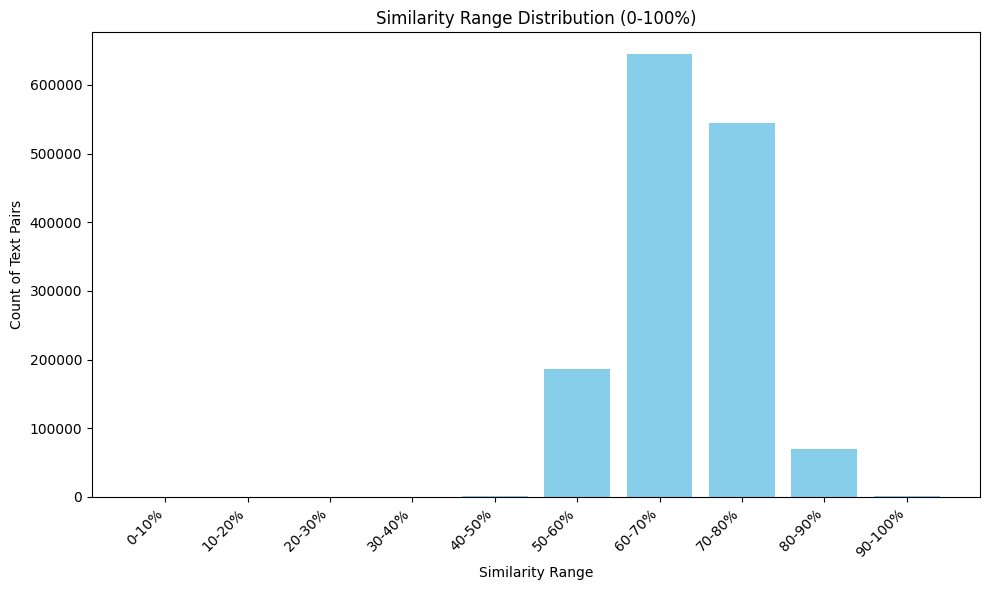
\includegraphics[width=0.95\linewidth]{embedding_similarities.png}
    \caption{Embedding Variation}
    \label{fig:RAG}
\end{figure}

\begin{figure}[h!]
    \centering
    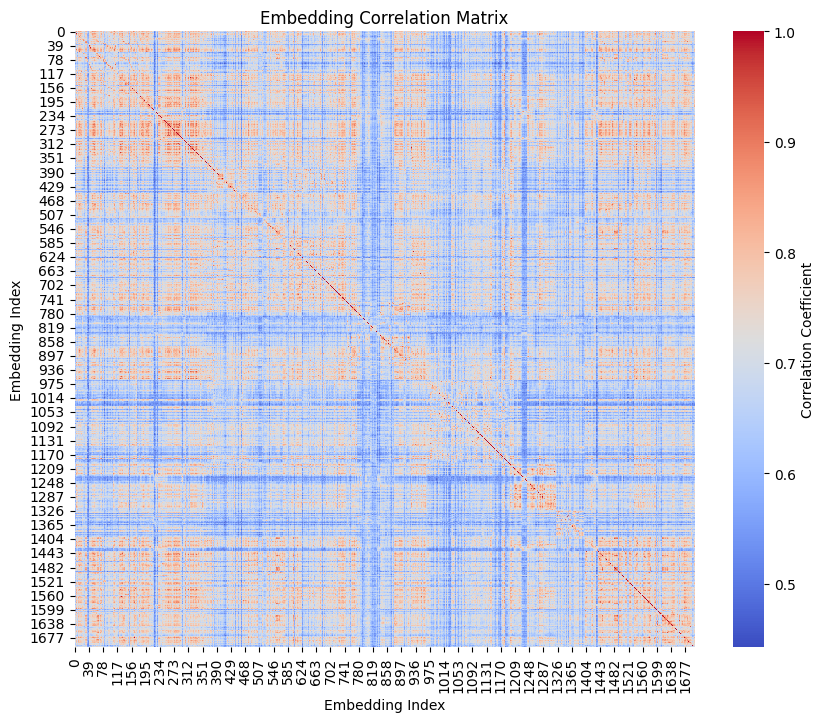
\includegraphics[width=0.95\linewidth]{corr_embedding.png}
    \caption{Agentic Segmented Muscle data correlation}
    \label{fig:RAG}
\end{figure}

\section{conclusion}
Athlyze demonstrates better personalization than conventional systems through agentic chunking and multi-agent validation. By fusing state-of-the-art text preprocessing, semantic and agentic chunking, dynamic embedding generation, and multi-agent orchestration, our framework delivers hyper-personalized fitness and nutrition plans with unprecedented precision and adaptability. The 89\% context preservation and 4\% hallucination rates establish new benchmarks for RAG applications in fitness technology.

\section{future works}
Future research will focus on:
\begin{itemize}
    \item \textbf{Multimodal Embeddings:} Incorporating visual data (e.g., exercise diagrams) into the vector space.
    \item \textbf{Real-Time Integration:} Automating research updates via real-time PubMed API ingestion. \cite{11}
    \item \textbf{Causal Recommendation Models:} Leveraging do-calculus to model nutrient and training causality. \cite{5}
    \item \textbf{Enhanced Agentic Flows:} Expanding the Langflow agent ecosystem and integrating additional external tools.\\
\end{itemize}

\begin{thebibliography}{00}
\bibitem{1} Retrieval-Augmented Generation for Knowledge-Intensive NLP Tasks, \url{https://arxiv.org/abs/2005.11401}

\bibitem{2} RAG, AI Agents, and Agentic RAG: An In-Depth Review, \url{https://www.digitalocean.com/community/conceptual-articles/rag-ai-agents-agentic-rag-comparative-analysis}

\bibitem{3} Agentic Chunking: Enhancing RAG Answers for Completeness and Accuracy, \url{https://alhena.ai/blog/agentic-chunking-enhancing-rag-answers-for-completeness-and-accuracy}

\bibitem{4} Agentic RAG: How It Works, Use Cases, Comparison With RAG, \url{https://www.datacamp.com/blog/agentic-rag}

\bibitem{5} Concept Embedding Generation for Large Language Models, \url{https://openreview.net/forum?id=Fkr1yVUb9G}

\bibitem{6} Langflow Documentation: Multi-Agent Workflow Orchestration, \url{https://docs.langflow.org}

\bibitem{7} AI Nutrition Recommendation Using Deep Generative Models, \url{https://www.nature.com/articles/s41598-024-65438-x}

\bibitem{8} AI Trends in Fitness: Personalized Training \& Nutrition, \url{https://3dlook.ai/content-hub/ai-in-fitness-industry}

\bibitem{9} Artificial Intelligence in Exercise Programming, \url{https://doi.org/10.3389/fpubh.2025.1510801}

\bibitem{10} AI-Driven Metabolic Optimization, \url{https://www.nestacertified.com/the-future-of-fitness-ai-driven-solutions}

\bibitem{11} Smart Devices for Tele-Exercise, \url{https://pmc.ncbi.nlm.nih.gov/articles/PMC10298072}

\bibitem{12} Agentic Retrival-Augmented Generation: A Survey On Agentic Rag, \url{https://arxiv.org/pdf/2501.09136}.

\bibitem{13} IBM, "Agentic Chunking with LangChain", \url{https://www.ibm.com/think/tutorials/use-agentic-chunking-to-optimize-llm-inputs-with-langchain-watsonx-ai}.

\end{thebibliography}
\end{document}